\chapter{Arhitektura i dizajn sustava}
			
			
			Odabir odgovarajuće arhitekture je važna odluka koja utječe na cjelokupnu funkcionalnost sustava. Budući da je cilj aplikacije široka dostupnost, odabrali smo web aplikaciju. Web aplikacija funkcionira neovisno o platformi, što oslobađa razvojni tim višeplatformnog razvoja.\\
			Korisnik aplikaciji pristupa pomoću web preglednika. Web preglednik je program koji omogućava korisniku pregled i prikaz web aplikacije na uređaju. Kako bi se omogućila komunikacija klijenta(korisnika) s aplikacijom koristi se web poslužitelj koji koristi HTTP protokol. Aplikacija komunicira sa backend-om preko REST API-ja. Backend dohvaća sve potrebne podatke iz baze podataka(više o njoj u sljedećoj sekciji) nakon čega preko poslužitelja i preglednika prikazuje te podatke korisniku u obliku HTML dokumenta.\\
			Aplikacija je pisana u programskom jeziku Java i programskom okruženju Spring Boot, te React-u(JavaScript biblioteka za izgradnju korisničkih sučelja), a od razvojnih okruženja odabrali smo Visual Studio Code za frontend  te IntelliJ IDEA za ostatak posla.\\
			
Logika backenda izgrađena je na temelju REST konvencije, stoga je razrađena u tri sloja: Repository, Service i Controller. 
			\begin{itemize}
				\item \textbf{Repository} – Sloj Repository primarno je zadužen za komunikaciju s bazom podataka. U njemu se nalaze standardne metode za dohvaćanje, spremanje i izmjenu podataka u bazi. Te metode temelje se na atributima entiteta za koji je izgrađen pojedini repository. Također, svaki repository može biti nadopunjen vlastitim metodama.
				\item \textbf{Service} – U Service sloju odvija se poslovna logika i manipulacija podacima koji dolaze s baze. To uključuje kreiranje klasa, promjenu tipova, omatanje i sl. 
				\item \textbf{Controller} –  prima i obrađuje zahtjeve poslužitelja. Svi se zahtjevi prosljeđuju koristeći JSON format. Shodno pojedinom zahtjevu, controller zatražuje podatke sa repositoryja, izvodi metode koje mu pruža Service. Na kraju podatke u obliku objekata šalje kao odgovor web poslužitelju.  
			\end{itemize}
			React je javascript knjižnica za izgradnju korisničkih sučelja. Temelji se na deklariranju komponenata koje se prikazuju korisniku preko web preglednika.
			\begin{figure}
				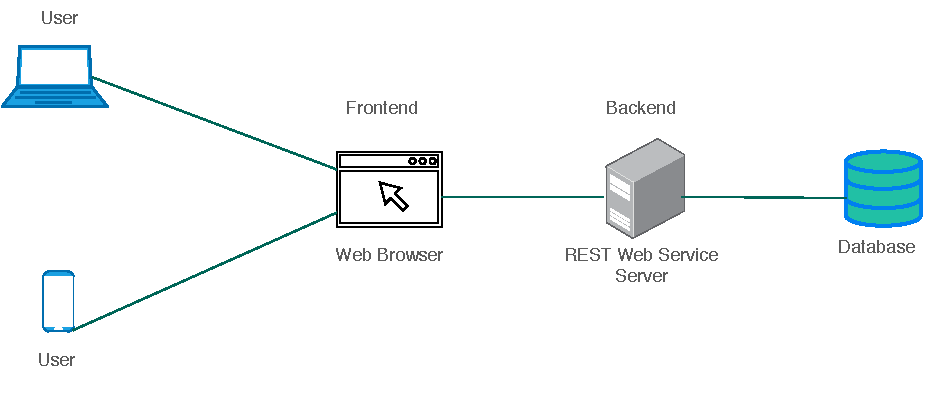
\includegraphics{Arhitektura_sustava}
				\caption{Arhitektura sustava}
			\end{figure}
			
			
			
			\section{Baza podataka}
			
			Sve je podatke potrebno negdje spremiti kako bi se mogli dinamički dohvaćati. Za ovo nam služi baza podataka, koju također smatramo dijelom MVC obrasca. Naša aplikacija u pozadini koristi, kao relacijsku bazu podataka, PostgreSQL.
			\\
			U bazi podataka nalaze se sljedeći entiteti:
			\begin{itemize}
				\item Korisnik
				\item Adresa
				\item Ocjena
				\item Zahtjev
				\item Potencijalni
			\end{itemize}
			
			\subsection{Opis tablica}
			
			
			\textbf{Korisnik} Ovaj entitet modelira jednog korisnika aplikacije.\\
			Sadrži atribute: korisnikID, ime, prezime, e-posta, lozinka, korisnickoIme, jeAdmin, telefon, slika, status, vrijemeBlokiranja i
			adresaID koji predstavlja strani ključ na entitet Adresa. Korisnik je povezan s entitetom Ocjena vezama "prima" i "daje" (\textit{One-to-Many}) preko atributa korisnikID. Korisnik se također veže s entitetom Zahtjev vezama "autorski" i "izvršiteljski" (\textit{One-to-Many}) preko atributa korisnikID i vezom "potencijalni" (\textit{Many-to-Many}) preko atributa korisnikID. Ovaj entitet se još veže uz entitet Adresa vezom \textit{Many-to-One} preko atributa korisnikID.
			
			\begin{tabularx} {\textwidth} {|p{3.5cm}|p{2cm}|X|}
				
				\hline
				\multicolumn{3}{|c|}{\textbf{Korisnik}} \\
				\hline

				
				\cellcolor{LightGreen}korisnikID & INT	&   jedinstveni identifikator svakog korisnika 	\\ \hline
				ime	& VARCHAR &   ime korisnika	\\ \hline 
				prezime & VARCHAR &  prezime korisnika \\ \hline 
				e-posta & VARCHAR	&  	e-mail adresa korisnika	\\ \hline 
				lozinka & VARCHAR	&  	hash lozinke	\\ \hline
				korisnickoIme & VARCHAR	&  	korisnicko ime	\\ \hline
				jeAdmin & BOOLEAN	&  	oznaka je li korisnik administrator	\\ \hline
				telefon & VARCHAR	&  	broj mobitela korisnika	\\ \hline
				slika & BOOLEAN	&  	oznaka je li korisnik ima sliku profila	\\ \hline
				status & VARCHAR	&  	oznaka statusa korisničkog računa	\\ \hline
				vrijemeBlokiranja & DATETIME	&  vrijeme blokiranja korisnika		\\ \hline
				\cellcolor{LightBlue}adresaId & VARCHAR	&  	adresa prebivališta korisnika	\\ \hline
				
				
				
			\end{tabularx} 
			
			\bigskip
			\bigskip
			\textbf{Adresa} Ovaj entitet modelira adresu prebivališta pojedinog korisnika aplikacije.
			Sadrži sljedeće atribute: adresaID, ulica, broj, pbr, imeMjesto. Entitet Adresa je u vezi \textit{One-to-Many} s entitetom Zahtjev preko atributa adresaID i u vezi \textit{One-to-Many} s entitetom Korisnik pomoću atributa adresaID.
			\bigskip
			
			
			\begin{tabularx} {\textwidth} {|p{3.5cm}|p{2cm}|X|}

				\hline
				\multicolumn{3}{|c|}{\textbf{Adresa}} \\
				\hline
				
				\cellcolor{LightGreen}adresaID & INT	& jedinstveni adrese korisnika	\\ \hline
				ulica	& VARCHAR &  naziv ulice 	\\ \hline 
				broj & INT & kućanski broj  \\ \hline 
				pbr & VARCHAR	&  	poštanski broj mjesta	\\ \hline 
				imeMjesto & VARCHAR	&  naziv mjesta		\\ \hline
				
				
				
			\end{tabularx}
			
			\bigskip
			\bigskip
			\textbf{Ocjena} Ovaj entitet predstavlja ocjenu koju jedan korisnik daje drugome. Sadrži atribute: ocjenaID, komentar, ocjena, korisnikID, zahtjevID, primakorisnikID. Ovaj entite sadrži tri strana ključa, a to su: korisnikID(predstavlja korisnika koji ocjenjuje), primakorisnikID(predstavlja korisnika kojeg se ocjenjuje) i zahtjevID(predstavlja zahtjev koji se izvršava). Ocjena je u  dvije veze s entitetom Korisnik, a to su "prima" (\textit{Many-to-One}) i "daje" (\textit{Many-to-One}) preko atributa korisnikID. Ocjena se još veže uz Zahtjev vezom \textit{One-to-One} preko atributa zahtjevID. 
			\bigskip
			
			\begin{tabularx} {\textwidth} {|p{3.5cm}|p{2cm}|X|}
				
				\hline
				\multicolumn{3}{|c|}{\textbf{Ocjena}} \\
				\hline
				
				\cellcolor{LightGreen}ocjenaID & INT	& jedinstveni identifikator svake ocjene	\\ \hline
				komentar	& VARCHAR &  komentar kojeg korisnik ostavlja uz ocjenu 	\\ \hline 
				ocjena & INT & ocjena koju korisnik dodjeljuje  \\ \hline 
				\cellcolor{LightBlue} korisnikID	& INT &  korisnik koji ocjenjuje 	\\ \hline 
				\cellcolor{LightBlue} zahtjevID	& INT &  zahtjev koji se izvršava 	\\ \hline 
				\cellcolor{LightBlue} primakorisnikID	& INT &  korisnik kojeg se ocjenjuje 	\\ \hline 
				
			\end{tabularx}
			
			\bigskip
			\bigskip
			\textbf{Zahtjev} Ovaj entitet predstavlja jedan zahtjev kojeg korisnik aplikacije zadaje ili izvršava. Sadrži atribute:zahtjevID, opis, datumVrPocetka, trajanje, status, adresaID, korisnikID, autorskikorisnikID. Kao i entitet ocjena i ovaj entitet sadrži tri strana ključa: adresaID(predstavlja adresu korisnika koji je zadao zahtjev, nije obavezno kako bi se kreirao zahtjev), korisnikID(predstavlja izvršitelja zahtjeva) i autorskikorisnikID(predstavlja samog kreatora zahtjeva). Entitet je u vezi s Ocjenom preko veze \textit{One-to-One} pomoću atributa zahtjevID. Zahtjev se veže uz entitet Korisnik preko tri veze "autorski" (\textit{Many-to-One}), veze "izvršiteljski" (\textit{Many-to-One}) i veze "potencijalni" (\textit{Many-to-Many}) svaka preko atributa korisnikID. Još se veže uz entitet Adresa \textit{One-to-Many} preko atributa adresaID. 
			\bigskip
			
			\begin{tabularx} {\textwidth} {|p{3.5cm}|p{2cm}|X|}
				
				\hline
				\multicolumn{3}{|c|}{\textbf{Zahtjev}} \\
				\hline
				
				\cellcolor{LightGreen}zahtjevID & INT	& jedinstveni identifikator svakog zahtjeva	\\ \hline
				opis	& VARCHAR &  kratki opis zahtjeva 	\\ \hline 
				datumVrPocetka & DATETIME &  trenutak postavljanja zahtjeva na aplikaciju \\ \hline 
				trajanje & TIME	&  vremenski period u kojem se zahtjev može izvršiti		\\ \hline 
				status & VARCHAR & status zahtjeva  \\ \hline
				\cellcolor{LightBlue} adresaID	& INT &  adresa autora zahtjeva 	\\ \hline 
				\cellcolor{LightBlue} korisnikID	& INT &  izvršitelj zahtjeva 	\\ \hline
				\cellcolor{LightBlue} autorskikorisnikID	& INT &   autor zahtjeva	\\ \hline
				
				
			\end{tabularx}
			
			\bigskip
			\bigskip
			\textbf{Potencijalni} Ovaj entitet predstavlja sve potencijalne izvršitelje jednog zahtjeva. Sadrži atribute: zahtjevID, korisnikID. Oba atributa su strani ključevi. Prvi predstavlja zahtjev kojeg korisnik želi izvršiti, drugi predstavlja korisnika koji želi izvršit zahtjev. Ovaj entitet nastaje radi \textit{Many-to-Many} veze "potencijalni" između Zahtjeva i Korisnika.
			\bigskip
			
			\begin{tabularx}{\textwidth} {|p{2cm}|p{2cm}|X|}
				\hline
				\multicolumn{3}{|c|}{\textbf{Potencijalni}} \\
				\hline
				\cellcolor{LightGreen} zahtjevID & INT & zahtjev kojeg korisnik želi izvršiti \\
				\hline
				\cellcolor{LightGreen} korisnikID & INT & potencijalni izvršitelj zahtjeva \\
				\hline
			\end{tabularx}
			
			
			
			\newpage
 			\subsection{Dijagram baze podataka}
			Podcrtani elementi su ključevi, elementi koji imaju (O) nisu obavezni za unos u bazu podataka, elementi koji imaju (FK) su strani ključevi i elementi s oznakom (U) moraju biti jedinstveni.
			
			\begin{figure}[h]
				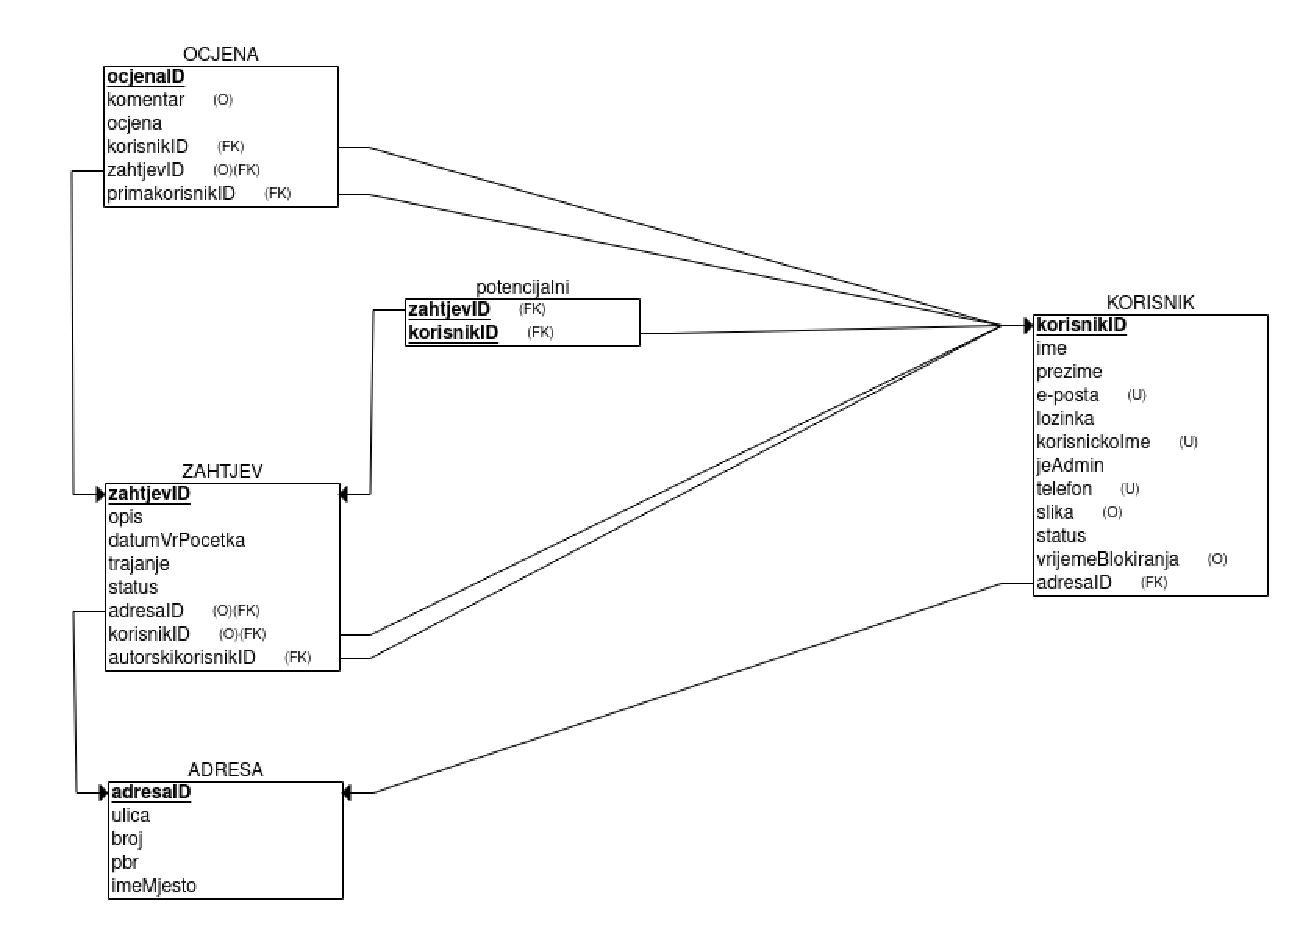
\includegraphics[height=0.53\textheight]{Relacijski_model}
				\caption{Relacijski model baze podataka}
			\end{figure}
			
			\eject

			
			
		\section{Dijagram razreda}
		
			U ovom poglavlju opisana je struktura \textit{backenda} aplikacije te opisana glavna funkcionalnost pojedinih klasa.\newline
			\newline
		
		
		
				Na slici 4.3 prikazana je konfiguracija aplikacije \textit{Pomozi mi}. Konfiguracija aplikacije temelji se na postavkama u klasi \textit{WebSecurity}, kojom su definiranja dopuštenja pristupa za pojedini \textit{path}, ponašanje pri \textit{loginu} i \textit{logoutu}. \\
				Klasom RestExceptionHandler regulirano je ponašanje sustava pri pojavi iznimke. Pojava iznimki rezultira \textit{responseom} u kojem je sadržana poruka iznimke.
				
				\begin{figure}[H]
					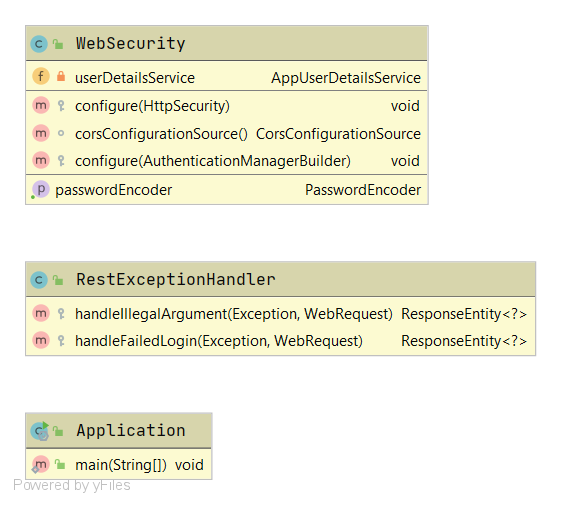
\includegraphics[scale=0.6]{slike/cs1.png} %veličina slike u odnosu na originalnu datoteku i pozicija slike
					\centering
					\caption{Struktura aplikacije i konfiguracija}
					
				\end{figure}
			
				\newpage
				
				Glavni preduvjet za obavljanje bilo kakve aktivnosti unutar aplikacije je da korisnik ima izrađen korisnički račun i prijavljen je u sustav. Klasom \textit{RegistrationDTO} modeliraju se podaci koje korisnik unosi prilikom registracije. Podaci takvog objekta služe kao predložak za stvaranje korisničkog računa. Za prijavu u sustav, provjeru korisničkog imena i lozinke te dodjeljivanje uloga zadužena je klasa \textit{AppUserDetailsService}. Korisniku može biti dodjeljena uloga ROLE\_USER i ROLE\_ADMIN kojima su određene ovlasti 
				slanja zahtjeva na kontrolere.
				
				
				\begin{figure}[H]
					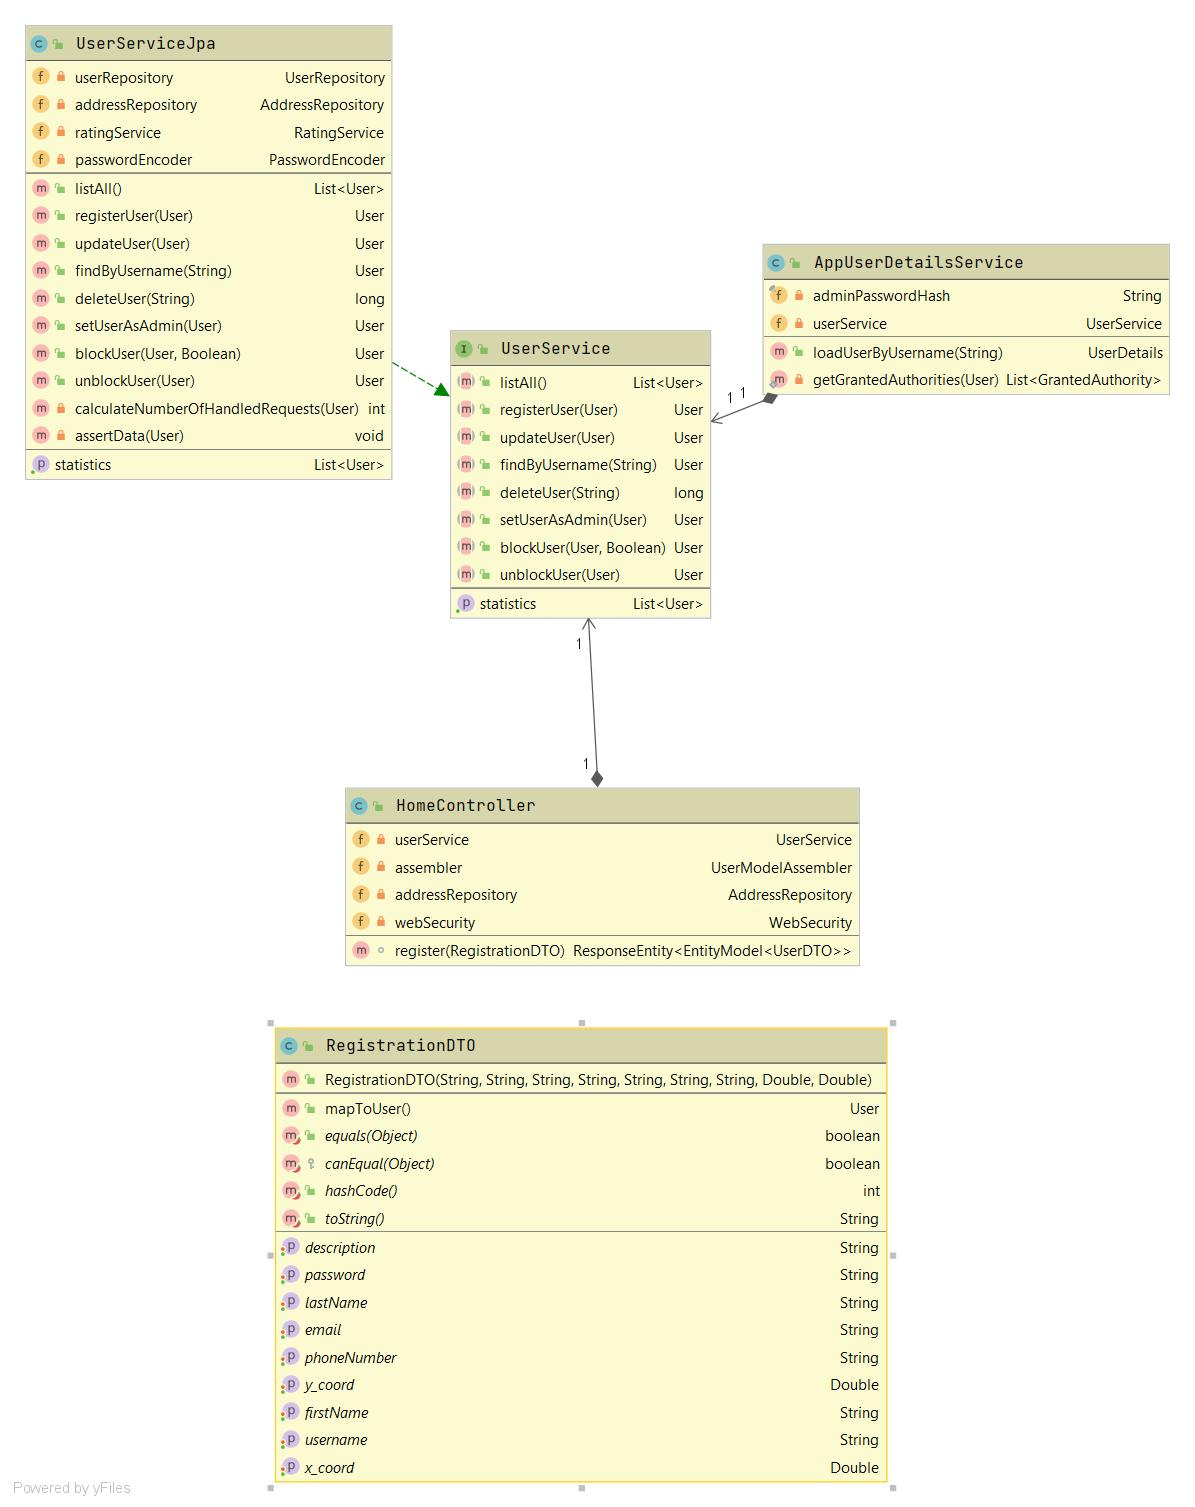
\includegraphics[scale=0.45]{slike/cs4.jpg} %veličina slike u odnosu na originalnu datoteku i pozicija slike
					\centering
					\caption{Klase koje reguliraju registraciju i prijavu}
					
				\end{figure}
			
				\newpage
				
				Slika 4.5 sadržava klase koje su ključne za aktivnosti i rad s korisnicima.
				Klasa \textit{User} predstavlja sam entitet kojim je opisan pojedini korisnik. Sadržava sve relevantne atribute za opis korisnika, konstruktore te funkciju \textit{mapToUserDTO} kojom se objekt \textit{User} pretvara u objekt pogodniji za komunikaciju sa \textit{frontendom}. \textit{UserDTO} predstavlja glavni model komunikacije s vanjskim korisnikom te skriva informacije o pojedinom \textit{Useru} koje nisu relevantne za prikaz na \textit{frontendu}.
				Omogućena je i pretvorba u suprotnom smjeru, iz klase \textit{UserDTO} u klasu \textit{User}. Klasa \textit{UserModelAssembler} omata klasu \textit{UserDTO} u oblik najprikladniji za interaktivnost prikaza, uključujući dodatne linkove. 
				Pristup i manipulacija zapisima korisnika u bazi podataka ostvaren je klasom \textit{UserRepository} koja sadrži sve standardne metode za rad sa zapisima.
				Poslovna logika koja se tiče korisnika ostvarena je u klasi \textit{UserServiceJpa}.
				\textit{UserController} zadužen je za obrađivanje zahtjeva. On inicijalizira komunikaciju sa servisom i bazom podataka i oblikuje podatke o korisnicima u odgovor na zahtjev.
				
				
			
				\begin{figure}[H]
				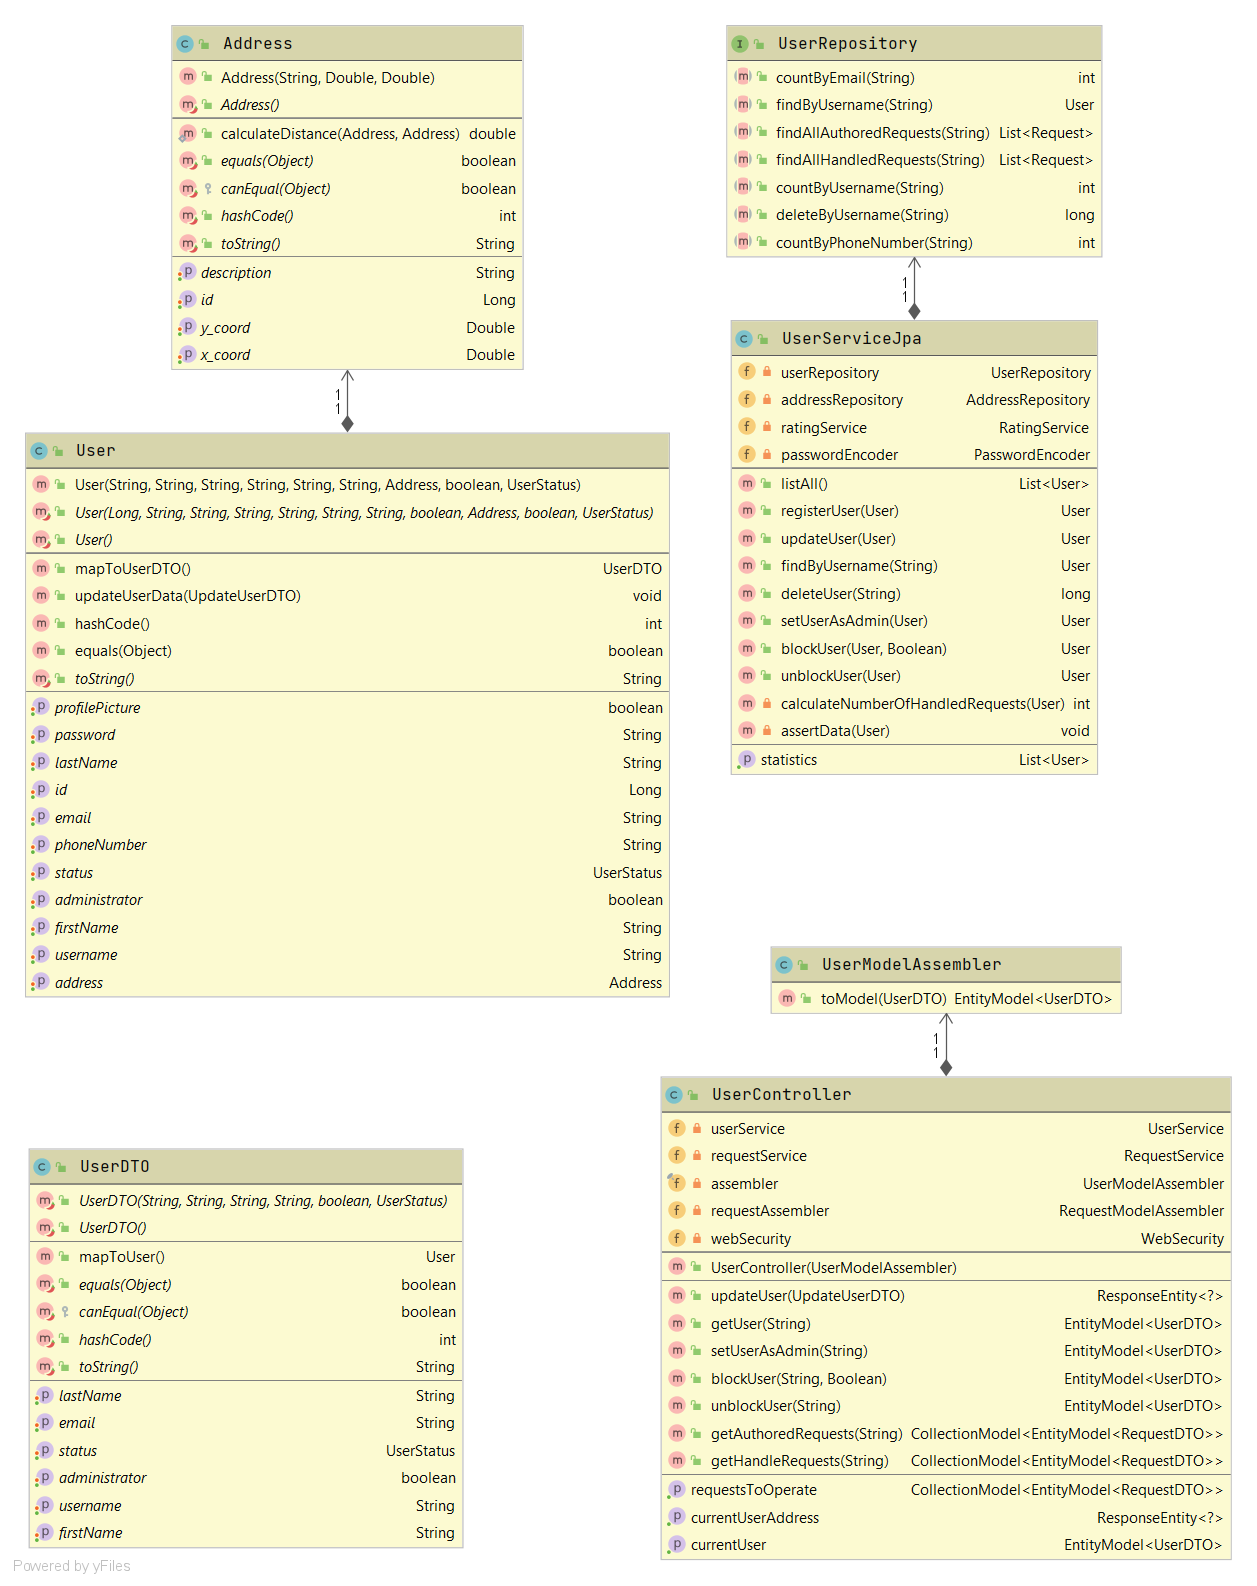
\includegraphics[scale=0.38]{slike/cs2.png} %veličina slike u odnosu na originalnu datoteku i pozicija slike
				\centering
				\caption{Klase koje reguliraju rad s korisnicima sustava}
				
				\end{figure}
			
				\newpage
				
				Klasa \textit{Request} modelira zahtjeve korisnika. Kao i u slučaju sa klasom \textit{User}, ova klasa ima pripadajuću klasu DTO-a, repozitorija, servisa i kontrolera. 
				Prilikom zadavanja zahtjeva, na kontoroler dolazi zahtjev koji u tijelu sadržava objekt tipa \textit{CreateRequestDTO} koji sadrži isključivo podatke koje unosi sam korisnik. Taj objekt je potrebno stvoriti objekt tipa \textit{Request} koristeći dobivene podatke i predefinirane podatke koji opisuju stanje zahtjeva kako bi se on mogao spremiti u bazu podataka.
				
				
			
				\begin{figure}[H]
					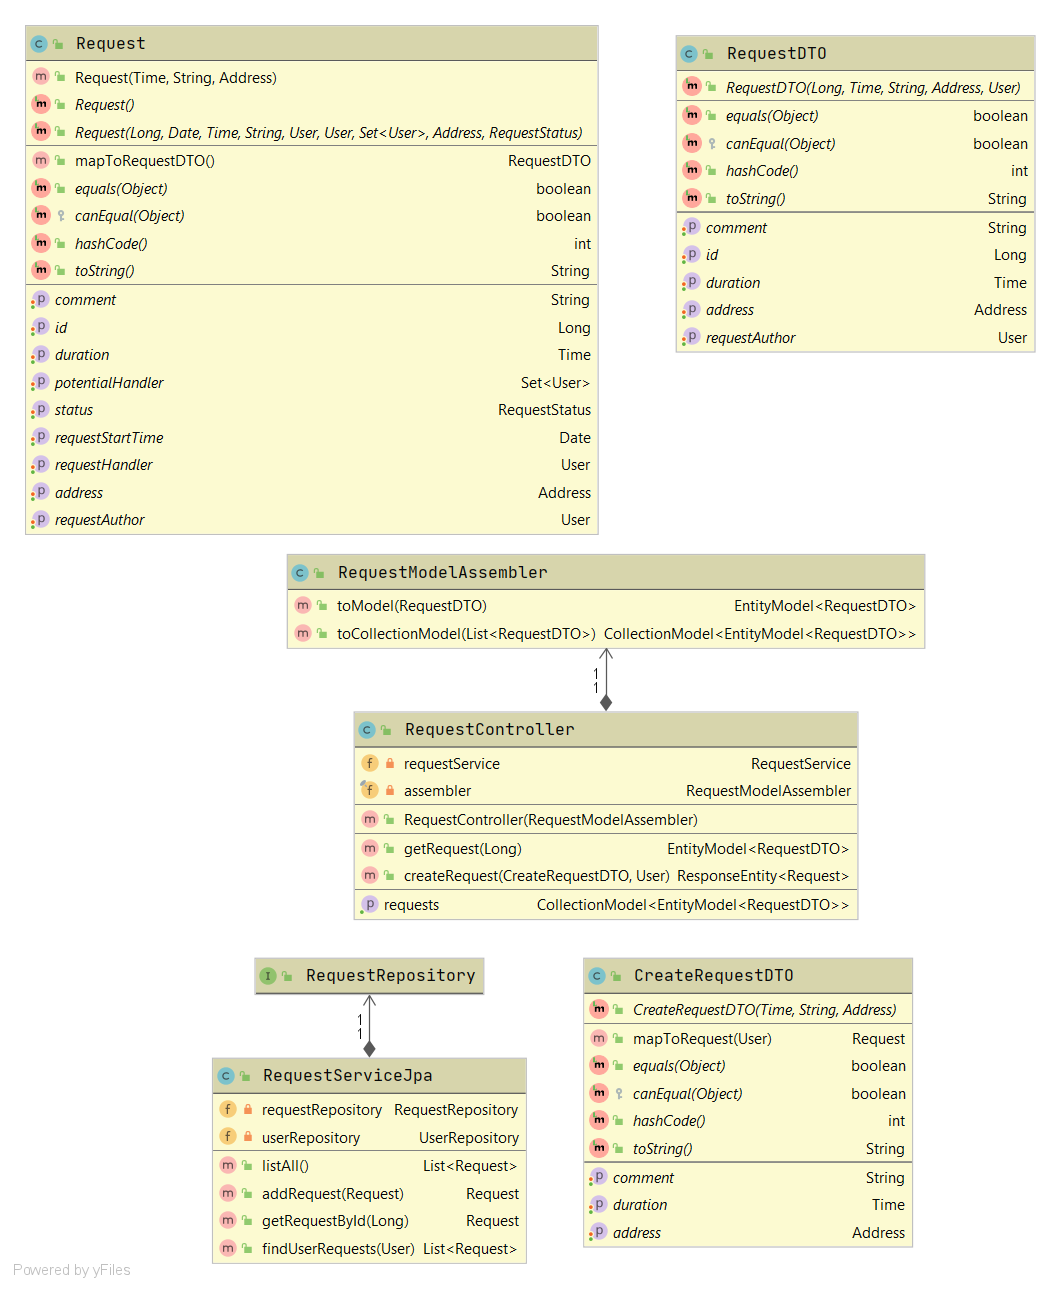
\includegraphics[scale=0.38]{slike/cs3.png} %veličina slike u odnosu na originalnu datoteku i pozicija slike
					\centering
					\caption{Klase koje reguliraju rad sa zahtjevima}
					
				\end{figure}
			
				\newpage
				
				Korisnicima je omogućeno međusobno ocjenjivanje te su na slici 4.7 prikazane klase koje služe modeliranju ocjena i ocjenjivanja. Svaka instancla klase \textit{RatingDTO} ima postavljenog korisnika koji je ocijenio te korisnika koji je ocjenjen,ocjenu, komentar te opcionalno zahtjev na koji se odnosi.
				\textit{RatingServiceJpa} omogućuje prikaz ocjena koje je pojedini korisnik autorirao te ocjena koje je pojedini korisnik dobio.			
				\begin{figure}[H]
					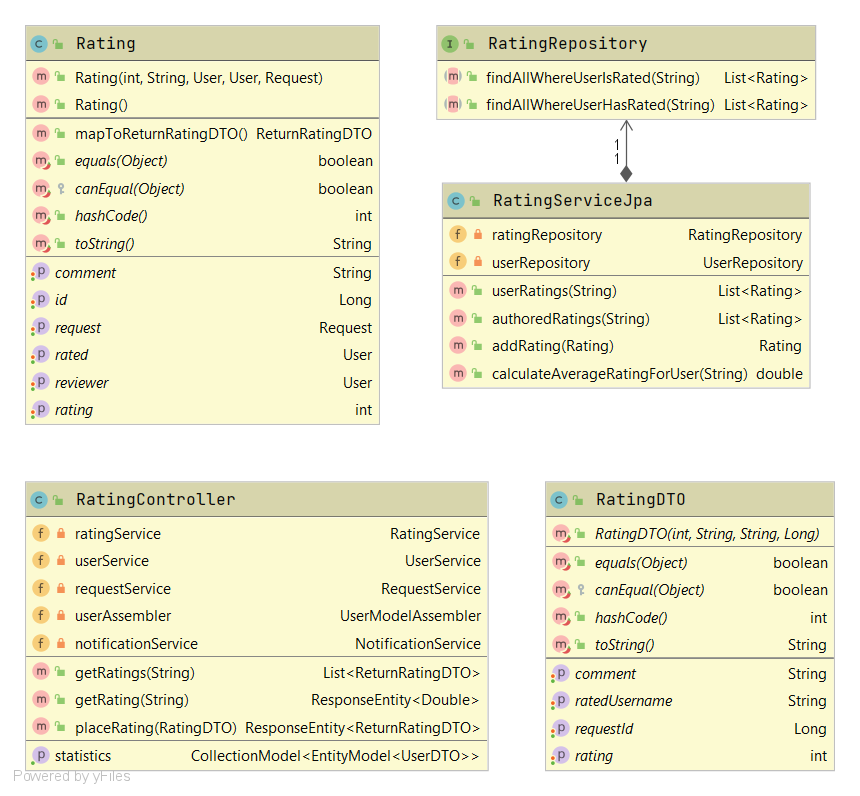
\includegraphics[scale=0.6]{slike/cs5.png} %veličina slike u odnosu na originalnu datoteku i pozicija slike
					\centering
					\caption{Klase koje reguliraju ocjenjivanje korisnika}
					
				\end{figure}
				
				
			
				
			
			
				
		
			
			
			\eject
		
		\section{Dijagram stanja}
			
			
			\textbf{\textit{dio 2. revizije}}\\
			
			\textit{Potrebno je priložiti dijagram stanja i opisati ga. Dovoljan je jedan dijagram stanja koji prikazuje \textbf{značajan dio funkcionalnosti} sustava. Na primjer, stanja korisničkog sučelja i tijek korištenja neke ključne funkcionalnosti jesu značajan dio sustava, a registracija i prijava nisu. }
			
			
			\eject 
		
		\section{Dijagram aktivnosti}
			
			\textbf{\textit{dio 2. revizije}}\\
			
			 \textit{Potrebno je priložiti dijagram aktivnosti s pripadajućim opisom. Dijagram aktivnosti treba prikazivati značajan dio sustava.}
			
			\eject
		\section{Dijagram komponenti}
		
			\textbf{\textit{dio 2. revizije}}\\
		
			 \textit{Potrebno je priložiti dijagram komponenti s pripadajućim opisom. Dijagram komponenti treba prikazivati strukturu cijele aplikacije.}